\chapter{Testiranje}

\section{Testiranje ekstrakcije fazora}

Testiranje ekstrakcije fazora se sastoji iz sljedećih koraka:

\begin{itemize}
    \item Definiranje signala od značaja (fundamentalne komponente)
    \item Superponiranje smetnji na fundamentalnu komponentu
    \item Propuštanje superponiranog signala kroz funkciju \textit{Ekstrakcija\_signala}
    \item Poređenje definiranog signala i ekstraktovanog signala
\end{itemize}

Signal na kojem se vrši testiranje (fundamentalna komponenta) je prikazan relacijom \ref{eq:41}. Prvo se testira djelovanje viših harmonika i bijelog šuma, a zatim djelovanje DC komponente. Grafici od značaja su prikazani u narednom poglavlju. 

\begin{equation}
    x(t) = 100\;sin(wt + \frac{\pi}{3})
    \label{eq:41}
\end{equation}


\section{Testiranje distantne zaštite}

Distantna zaštita se testira na signalima generisanim u \textit{Simulink} modelu prikazanim na slici \ref{fig:41}. Simulacija se izvodi sa fiksnim korakom koji je jednak unesenom periodu uzorkovanja. Mreža radi na frekvenciji od 50 Hz, a sastoji se od trofaznog simetričnog generatora u spoju $Y_g$ sa naponom između faza od 15000 V. Na generator je spojena linija ukupne dužine od 120 km, koja je podijeljena na 2 bloka (20 km + 100 km) kako bi se između njih mogao simulirati kvar. Sa \textit{Step} blokom se definiše u kojem trenutku djeluje kvar i podešeno je da traje kroz cijelu simulaciju. Linija je spojena na trofazni $Y_g$ potrošač aktivne snage 100000 W. Na početku linije je postavljen idealni mjerač napona i struja (faza-zemlja) za sve tri faze na koji se dodaje bijeli šum i koji se dovodi na AD kvantizator kako bi se simulirao uticaj tih komponenti, te se ti podaci eksportuju u \textit{workspace} i testiraju korištenjem GUI-a. Impedanse faza-faza nisu uzimane u razmatranje jer su se svi kvarovi manifestirali i na impedanse faza-zemlja. Generalno kod mreže je bitno poznavati osobine prilikom odabira AD konvertora kako ne bi došlo do zasićenja prilikom mjerenja koje bi dovelo do pogreške. Parametri linije su impedanse $Z_0$ i $Z_1$ (podužna nulta i pozitivna komponente) koje su potrebne za računanje udaljenosti.
\\ \\ 
Parametri AD kvantizatora:

\begin{itemize}
    \item Rezolucija : 16 bita
    \item Minimalna vrijednost: -20000
    \item Maksimalna vrijednost: 20000
\end{itemize}

Parametri linije:

\begin{itemize}
    \item $Z_0$ = 0.3864 + jw\;4.1264e-3
    \item $Z_1$ = 0.01273 + jw\;0.9337e-3
\end{itemize}

Nakon što se podese željeni parametri u \textit{Simulink} modelu i pokrene simulacija, potrebno je pokrenuti skriptu \textit{GenerisiPeriod.m} koja izdvaja vrijednosti struja ($I_a$, $I_b$, $I_c$) i napona ($U_a$, $U_b$, $U_c$) na odabranom periodu. Poželjno je odabrati što veću vrijednost perioda kako bi se izbjegli efekti startanja generatora koji unesu grešku prilikom računanja udaljenosti. Nakon toga je potrebno popuniti GUI i pokrenuti ga. Primjeri koji su navedeni u sljedećem poglavlju su priloženi u popratnom folderu \textit{Podaci} i mogu se učitati u workspace \textit{MATLAB-a}, pa onda popuniti GUI bez potrebe za pokretanjem \textit{Simulink} modela.

\begin{figure}[H]
  \centering
  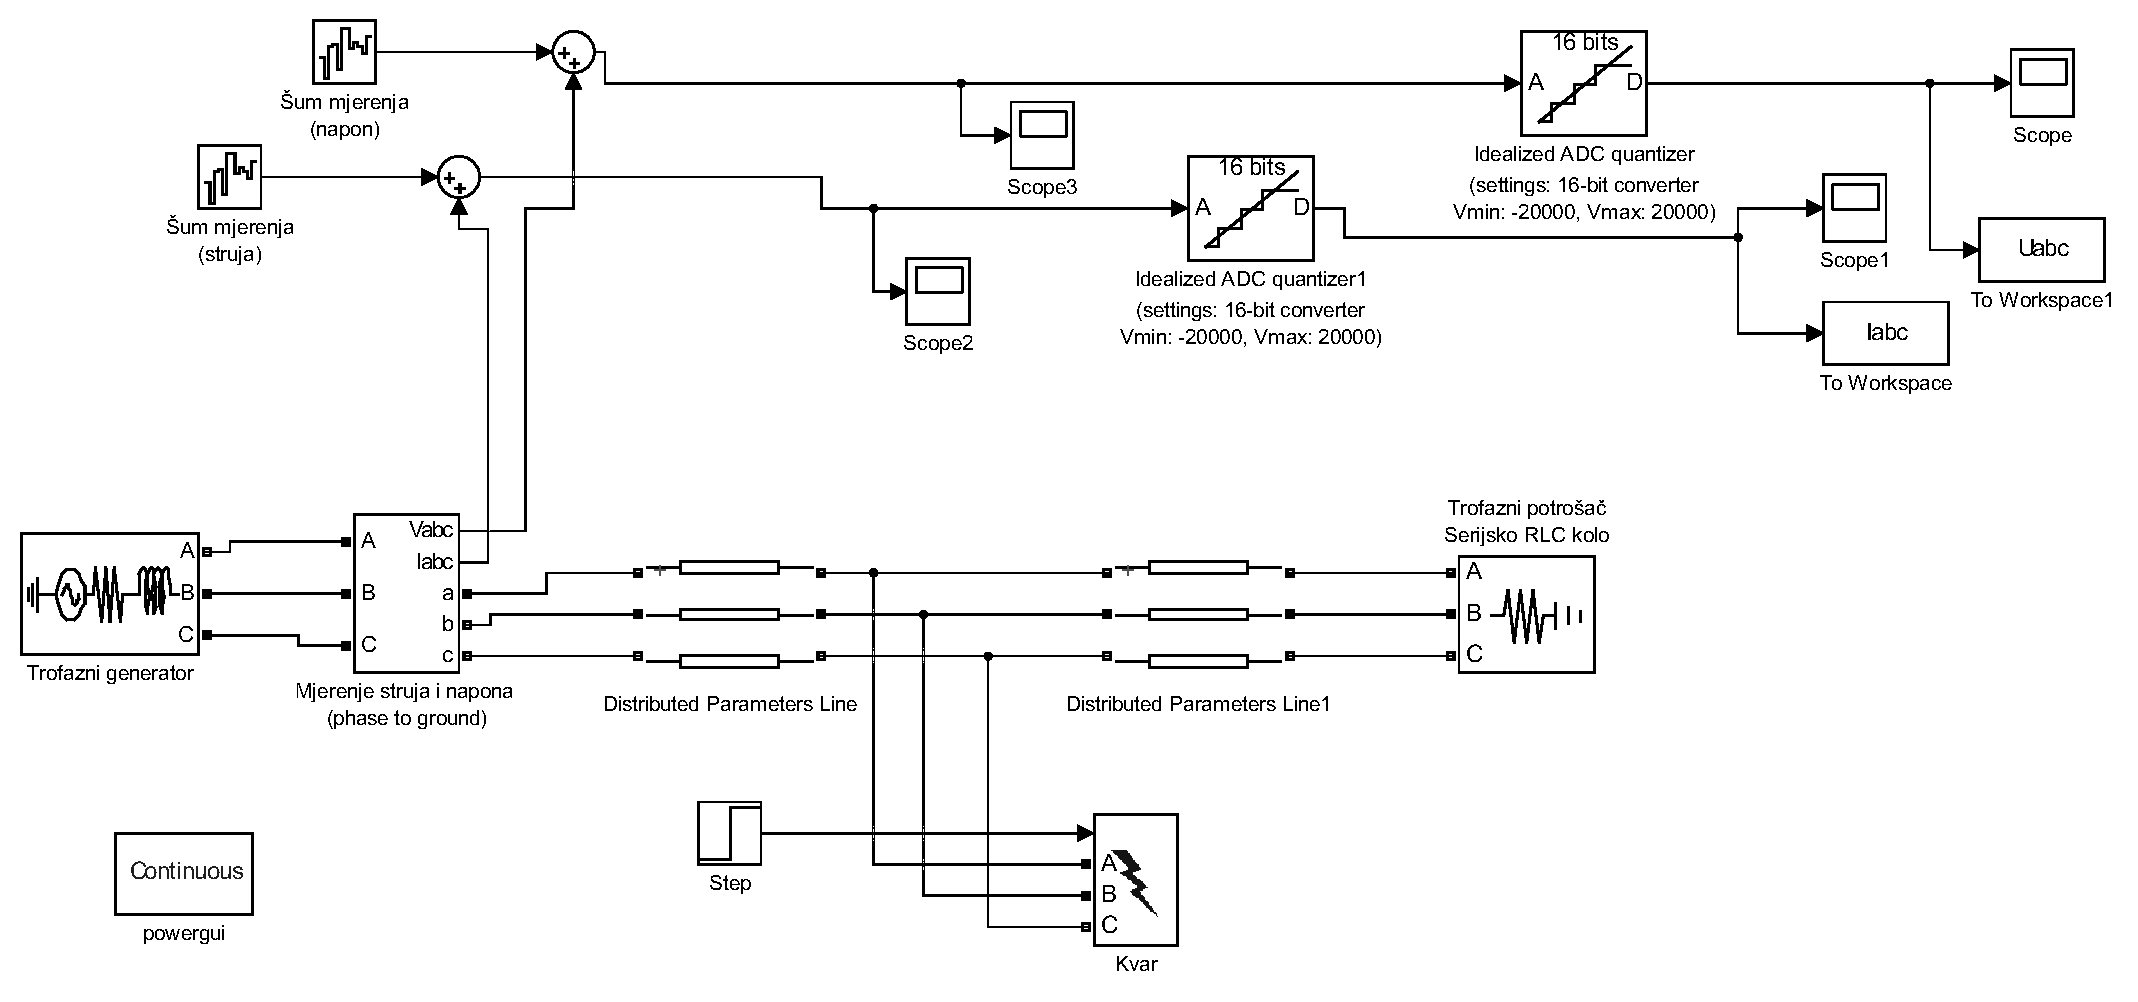
\includegraphics[width=1\textwidth]{Rezultati1/model_slika.eps}
  \caption{Simulink model mreže}
  \label{fig:41}
\end{figure}

